
%En ella se deben exponer brevemente pero con absoluta claridad, 
% la novedad y actualidad del tema,
% el objeto de la investigación,
% sus objetivos,
% la hipótesis de trabajo,
% el fundamento metodológico y
% los métodos utilizados para realizar el trabajo de investigación.
%Es decir, que la introducción es la fundamentación científica de la tesis en forma resumida.

\section{Introduction}
\begin{frame}

  The aim of this work is to support decision making regarding
  the location and redeployment of insurance agents to attend car wrecks.

  The idea is to develop models and methods for 
  (a) improving the service offered by insurance agents, 
  helping them arrive to the accident sites sooner, and 
  (b)  determining the number of adjusters required to perform 
  the service within the desired standards.

\end{frame}

\subsection{Problem}
\frame{
  The main goal is to determine the optimal bases (locations) 
  for placing the insurance company adjusters, 
  so as to minimize the average or maximum response time
  from customer calls when accidents occur.
  \begin{center}
    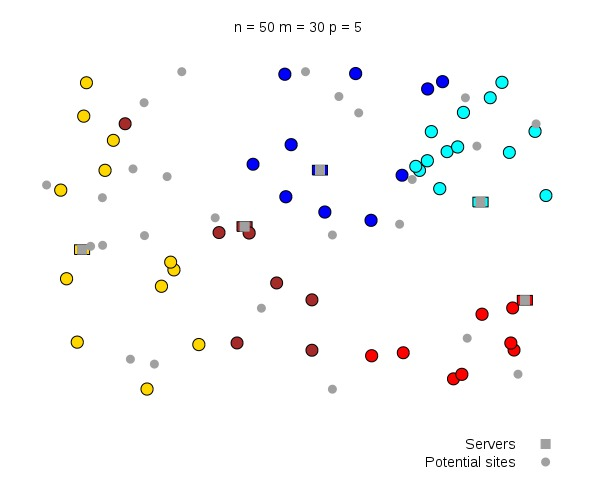
\includegraphics[scale=0.35]{SQpM_problem}
  \end{center}
}

\subsection{Motivation}
\begin{frame}
  When a car accident occurs, traffic congestion starts to pile up.
  This is because customers are not allowed to move their vehicles
  until the adjuster arrives.  
  The adjuster must record and determine the causes of the accident, 
  in order to move the car from the accident area and restore the flow.
  \begin{center}
    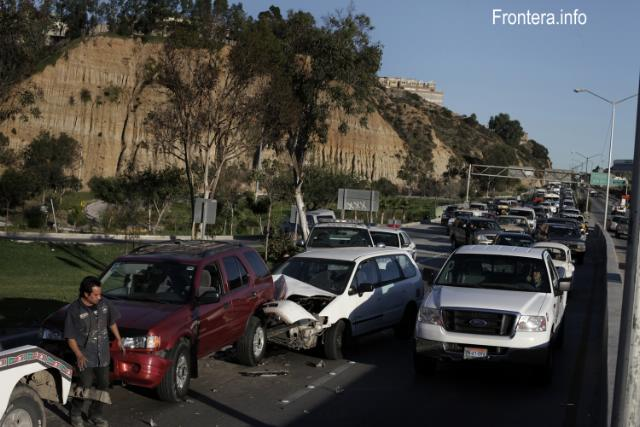
\includegraphics[scale=0.25]{389200-G}
  \end{center}
\end{frame}
